\documentclass[conference,10pt]{IEEEtran}
\usepackage[utf8]{inputenc}
\usepackage{graphicx}
\usepackage{amsmath}
\usepackage{booktabs}
\usepackage{multirow}
\usepackage{xcolor}
\usepackage[hidelinks]{hyperref}
\hypersetup{colorlinks=true,linkcolor=blue!70!black,citecolor=blue!70!black,urlcolor=blue!70!black}
\usepackage{float}
\usepackage{caption}
\usepackage{subcaption}
\usepackage{array}
\usepackage{cite}
\usepackage{textcomp}
\usepackage{balance}
\usepackage{tikz}
\usetikzlibrary{arrows.meta, positioning, calc, fit, backgrounds}

% Better table formatting
\renewcommand{\arraystretch}{1.15}

% Section formatting
\renewcommand\thesectiondis{\arabic{section}.}
\renewcommand\thesubsectiondis{\thesectiondis\arabic{subsection}.}

\title{Automated Industrial Environmental Compliance\\Monitoring Using Multi-Temporal Sentinel-2\\Imagery and Machine Learning Classification}

\author{
\IEEEauthorblockN{Oishik Kar, Mihir Dagar, Shouvik Das, Youvansh Chauhan}
\IEEEauthorblockA{Under the guidance of \textbf{Dr.\ Sunil C K}, Assistant Professor\\
Department of Computer Science and Engineering\\
Indian Institute of Information Technology (IIIT), Dharwad, Karnataka 580009, India\\
\textit{\{oishik, mihir, shouvik, youvansh\}@iiitdwd.ac.in}}
}

\begin{document}
\maketitle

\begin{abstract}
This paper presents an automated pipeline for monitoring environmental compliance in industrial zones using multi-temporal Sentinel-2 satellite imagery and supervised machine learning. We analyze two industrial areas in Bengaluru\textemdash Peenya and Whitefield\textemdash across a four-year observation period (2020 to 2024) to quantify green cover reduction and detect unauthorized construction activity. The proposed system integrates KGIS (Karnataka Geographic Information System) boundary data for study area delineation, programmatic Sentinel-2 data acquisition via the STAC API, spectral index computation (NDVI, NDBI, NBI), Random Forest classification achieving 97.7--98.7\% accuracy on held-out test sets, and automated violation extraction with geo-referenced coordinates. Experimental results indicate significant green cover loss of 24.1\% in Peenya and 27.8\% in Whitefield, with 126 geo-tagged violation zones identified across both regions. The modular pipeline architecture enables direct extension to arbitrary geographic areas, supporting scalable, continuous environmental surveillance for state pollution control boards.
\end{abstract}

\begin{IEEEkeywords}
Remote sensing, NDVI, change detection, land cover classification, Random Forest, Sentinel-2, environmental compliance, industrial monitoring, GIS
\end{IEEEkeywords}

\section{Introduction}

Industrial expansion in Indian metropolitan areas frequently occurs at the expense of mandated green belts and environmental buffers. The Karnataka State Pollution Control Board (KSPCB) requires industrial premises to maintain minimum green cover thresholds, yet manual monitoring through field inspections remains infrequent and operationally difficult to scale across hundreds of factory sites~\cite{cpcb2021}. Satellite-based remote sensing, with its combination of high temporal revisit rates (5-day cycle for Sentinel-2) and multispectral sensing capabilities, offers a viable pathway toward automated, continuous environmental surveillance.

This work addresses \textbf{Statement~3} of the Machine Learning course project: the design of a system that (i)~utilizes GIS boundary data to identify factory premises, (ii)~analyzes satellite imagery over time to detect reduction in green cover and unauthorized construction, (iii)~applies ML models for vegetation detection and land-use change classification, and (iv)~generates compliance reports with geo-tagged violation alerts, temporal change analysis, and annotated visual evidence.

\smallskip
\noindent The principal contributions of this work are:
\begin{enumerate}
    \item An end-to-end automated pipeline (Fig.~\ref{fig:arch}) spanning cloud-native data acquisition, spectral analysis, supervised and unsupervised classification, change detection, and compliance report generation.
    \item A Random Forest classifier trained exclusively on raw spectral features, achieving 97.7--98.7\% accuracy with a non-circular validation methodology that decouples training features from label generation.
    \item A quantitative compliance assessment of two major Bengaluru industrial zones over the 2020--2024 period, identifying 126 violation hotspots with precise geographic coordinates and area estimates.
\end{enumerate}

\begin{figure*}[t]
    \centering
    \resizebox{0.98\textwidth}{!}{
    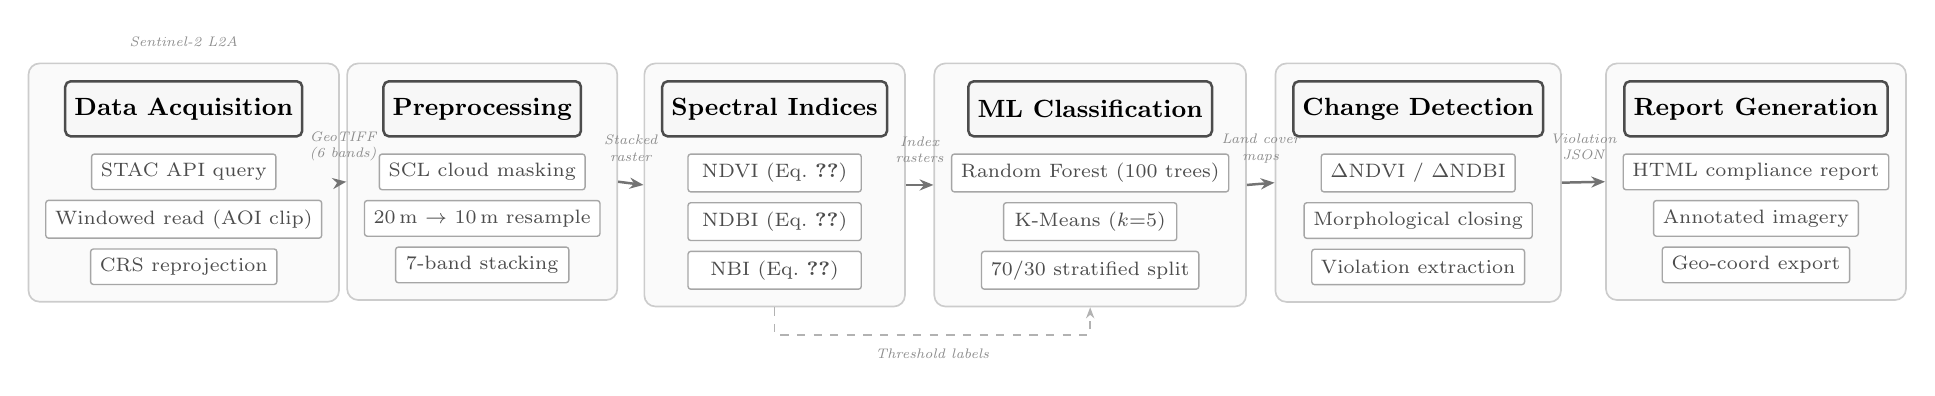
\begin{tikzpicture}[
        node distance=0.3cm and 0.35cm,
        stage/.style={
            rectangle, rounded corners=2pt, draw=black!70, line width=0.9pt,
            fill=black!3, minimum width=2.4cm, minimum height=0.7cm,
            align=center, font=\small\bfseries
        },
        sub/.style={
            rectangle, rounded corners=1pt, draw=black!35, line width=0.5pt,
            fill=white, minimum width=2.2cm, minimum height=0.45cm,
            align=center, font=\scriptsize, text=black!70
        },
        arr/.style={-{Stealth[length=5pt, width=4pt]}, line width=0.9pt, black!55},
        dataarr/.style={-{Stealth[length=4pt, width=3pt]}, line width=0.5pt, black!30, dashed},
        datalbl/.style={font=\tiny\itshape, text=black!45, align=center},
        grp/.style={rectangle, rounded corners=4pt, draw=black!20, line width=0.6pt,
            fill=black!2, inner sep=6pt}
    ]
    % === Stage 1: Data Acquisition ===
    \node[stage] (s1) {Data Acquisition};
    \node[sub, below=0.2cm of s1] (s1a) {STAC API query};
    \node[sub, below=0.12cm of s1a] (s1b) {Windowed read (AOI clip)};
    \node[sub, below=0.12cm of s1b] (s1c) {CRS reprojection};
    \begin{scope}[on background layer]
        \node[grp, fit=(s1)(s1a)(s1b)(s1c)] (g1) {};
    \end{scope}

    % === Stage 2: Preprocessing ===
    \node[stage, right=1.0cm of s1] (s2) {Preprocessing};
    \node[sub, below=0.2cm of s2] (s2a) {SCL cloud masking};
    \node[sub, below=0.12cm of s2a] (s2b) {20\,m $\to$ 10\,m resample};
    \node[sub, below=0.12cm of s2b] (s2c) {7-band stacking};
    \begin{scope}[on background layer]
        \node[grp, fit=(s2)(s2a)(s2b)(s2c)] (g2) {};
    \end{scope}

    % === Stage 3: Spectral Indices ===
    \node[stage, right=1.0cm of s2] (s3) {Spectral Indices};
    \node[sub, below=0.2cm of s3] (s3a) {NDVI (Eq.~\ref{eq:ndvi})};
    \node[sub, below=0.12cm of s3a] (s3b) {NDBI (Eq.~\ref{eq:ndbi})};
    \node[sub, below=0.12cm of s3b] (s3c) {NBI (Eq.~\ref{eq:nbi})};
    \begin{scope}[on background layer]
        \node[grp, fit=(s3)(s3a)(s3b)(s3c)] (g3) {};
    \end{scope}

    % === Stage 4: ML Classification ===
    \node[stage, right=1.0cm of s3] (s4) {ML Classification};
    \node[sub, below=0.2cm of s4] (s4a) {Random Forest (100 trees)};
    \node[sub, below=0.12cm of s4a] (s4b) {K-Means ($k{=}5$)};
    \node[sub, below=0.12cm of s4b] (s4c) {70/30 stratified split};
    \begin{scope}[on background layer]
        \node[grp, fit=(s4)(s4a)(s4b)(s4c)] (g4) {};
    \end{scope}

    % === Stage 5: Change Detection ===
    \node[stage, right=1.0cm of s4] (s5) {Change Detection};
    \node[sub, below=0.2cm of s5] (s5a) {$\Delta$NDVI / $\Delta$NDBI};
    \node[sub, below=0.12cm of s5a] (s5b) {Morphological closing};
    \node[sub, below=0.12cm of s5b] (s5c) {Violation extraction};
    \begin{scope}[on background layer]
        \node[grp, fit=(s5)(s5a)(s5b)(s5c)] (g5) {};
    \end{scope}

    % === Stage 6: Reporting ===
    \node[stage, right=1.0cm of s5] (s6) {Report Generation};
    \node[sub, below=0.2cm of s6] (s6a) {HTML compliance report};
    \node[sub, below=0.12cm of s6a] (s6b) {Annotated imagery};
    \node[sub, below=0.12cm of s6b] (s6c) {Geo-coord export};
    \begin{scope}[on background layer]
        \node[grp, fit=(s6)(s6a)(s6b)(s6c)] (g6) {};
    \end{scope}

    % === Main flow arrows ===
    \draw[arr] (g1.east) -- (g2.west);
    \draw[arr] (g2.east) -- (g3.west);
    \draw[arr] (g3.east) -- (g4.west);
    \draw[arr] (g4.east) -- (g5.west);
    \draw[arr] (g5.east) -- (g6.west);

    % === Data flow labels ===
    \node[datalbl, above=0.08cm of g1] {Sentinel-2 L2A};
    \node[datalbl] at ($(g1.east)!0.5!(g2.west)+(0,0.45)$) {GeoTIFF\\(6 bands)};
    \node[datalbl] at ($(g2.east)!0.5!(g3.west)+(0,0.45)$) {Stacked\\raster};
    \node[datalbl] at ($(g3.east)!0.5!(g4.west)+(0,0.45)$) {Index\\rasters};
    \node[datalbl] at ($(g4.east)!0.5!(g5.west)+(0,0.45)$) {Land cover\\maps};
    \node[datalbl] at ($(g5.east)!0.5!(g6.west)+(0,0.45)$) {Violation\\JSON};

    % === Label generation feedback ===
    \draw[dataarr] (g3.south) -- ++(0,-0.35) -| node[datalbl, pos=0.25, below=0.05cm] {Threshold labels} (g4.south);

    \end{tikzpicture}
    }
    \caption{Detailed system architecture. Each stage (bold header) contains specific sub-processes. The dashed feedback path shows how spectral indices generate threshold-based pseudo-labels consumed by the ML classification stage, while the classifier itself trains on raw spectral bands only (non-circular design).}
    \label{fig:arch}
\end{figure*}

\section{Study Area and Data}

\subsection{Study Zones}

Two industrial areas in Bengaluru, Karnataka were selected for this study (Fig.~\ref{fig:beforeafter}).

\noindent\textbf{Peenya Industrial Area} (13.01--13.07\textdegree{}N, 77.48--77.56\textdegree{}E) is one of the largest industrial estates in South Asia, spanning approximately 40~km\textsuperscript{2} with over 8,000 registered manufacturing, electronics, and heavy industry units.

\noindent\textbf{Whitefield Industrial Area} (12.95--13.01\textdegree{}N, 77.72--77.80\textdegree{}E) is a rapidly urbanizing IT corridor with mixed industrial and residential development, covering approximately 25~km\textsuperscript{2}. Both zones have experienced significant land-use transitions driven by Bengaluru's rapid metropolitan expansion.

\subsection{Satellite Data}

We acquired Sentinel-2 Level-2A (L2A) surface reflectance imagery from the Microsoft Planetary Computer~\cite{pc2023} via the SpatioTemporal Asset Catalog (STAC) API. The L2A product provides bottom-of-atmosphere (BOA) reflectance corrected by the Sen2Cor processor~\cite{drusch2012}, suitable for quantitative multitemporal analysis. Two cloud-free acquisition dates were selected during the dry season (January--March) to minimize atmospheric interference and seasonal vegetation variability:

\begin{table}[h]
\centering
\caption{Sentinel-2 Acquisition Parameters}
\label{tab:acq}
\begin{tabular}{lcc}
\toprule
\textbf{Parameter} & \textbf{T1 (Baseline)} & \textbf{T2 (Recent)} \\
\midrule
Acquisition Date & March 2020 & March 2024 \\
Cloud Cover & $<$0.2\% & $<$0.01\% \\
Processing Level & L2A (BOA) & L2A (BOA) \\
\bottomrule
\end{tabular}
\end{table}

Six spectral bands were acquired per period, as detailed in Table~\ref{tab:bands}. Bands at 20\,m native resolution (B11, B12) were resampled to 10\,m using bilinear interpolation to produce spatially uniform composites. The Scene Classification Layer (SCL) was obtained for pixel-level cloud and shadow masking. The complete dataset comprises \textbf{11.6~million multispectral pixels} across 28 Cloud-Optimized GeoTIFF files.

\begin{table}[h]
\centering
\caption{Spectral Bands Used in Analysis}
\label{tab:bands}
\begin{tabular}{llcc}
\toprule
\textbf{Band} & \textbf{Name} & \textbf{$\lambda$ (nm)} & \textbf{Res.\ (m)} \\
\midrule
B02 & Blue & 490 & 10 \\
B03 & Green & 560 & 10 \\
B04 & Red & 665 & 10 \\
B08 & NIR & 842 & 10 \\
B11 & SWIR-1 & 1610 & 20$\to$10 \\
B12 & SWIR-2 & 2190 & 20$\to$10 \\
SCL & Scene Class & -- & 20$\to$10 \\
\bottomrule
\end{tabular}
\end{table}

Study area delineation was performed using administrative boundary shapefiles obtained from the Karnataka Geographic Information System (K-GIS) portal~\cite{kgis2024}, operated by KSRSAC. Specifically, Taluk-level boundaries for Bangalore-North (code~2001, encompassing Peenya) and Bangalore-East (code~2004, encompassing Whitefield) were downloaded as ESRI Shapefiles, reprojected from UTM Zone~43N to WGS84, and exported as GeoJSON polygons for integration with the satellite data pipeline. Ward-level administrative metadata for each violation location was further verified using the K-GIS Location Details REST API (\texttt{getlocationdetails}).

\section{Methodology}

The proposed system follows a six-stage pipeline architecture (Fig.~\ref{fig:arch}). Each stage is implemented as an independent, reusable Python module.

\subsection{Preprocessing}

Raw spectral bands are stacked into 7-band composites (B02, B03, B04, B08, B11, B12, cloud mask). Cloud and shadow pixels are masked using the SCL band: classes~3 (cloud shadow), 8 (medium-probability cloud), 9 (high-probability cloud), and 10 (thin cirrus) are flagged invalid. Valid pixel coverage exceeded \textbf{99.8\%} across all four acquisitions, confirming the effectiveness of dry-season temporal selection.

\subsection{Spectral Index Computation}

Three spectral indices are computed for each time period:

\noindent\textbf{NDVI}~\cite{rouse1974} quantifies photosynthetically active vegetation:
\begin{equation}
    \text{NDVI} = \frac{\rho_{\text{NIR}} - \rho_{\text{Red}}}{\rho_{\text{NIR}} + \rho_{\text{Red}}} \label{eq:ndvi}
\end{equation}

\noindent\textbf{NDBI}~\cite{zha2003} captures urban impervious surfaces:
\begin{equation}
    \text{NDBI} = \frac{\rho_{\text{SWIR1}} - \rho_{\text{NIR}}}{\rho_{\text{SWIR1}} + \rho_{\text{NIR}}} \label{eq:ndbi}
\end{equation}

\noindent\textbf{NBI} provides sensitivity to bare soil and fresh construction:
\begin{equation}
    \text{NBI} = \frac{\rho_{\text{Red}} \times \rho_{\text{SWIR1}}}{\rho_{\text{NIR}}} \label{eq:nbi}
\end{equation}

\subsection{Change Detection}

Bitemporal differencing yields $\Delta\text{NDVI} = \text{NDVI}_{T2} - \text{NDVI}_{T1}$ and $\Delta\text{NDBI} = \text{NDBI}_{T2} - \text{NDBI}_{T1}$. A composite 4-class change mask is generated using thresholds derived from established literature~\cite{zha2003}:
\begin{equation}
\text{Class} = \begin{cases}
    1 & \text{if } \Delta\text{NDVI} < -0.15 \quad (\text{vegetation loss}) \\
    2 & \text{if } \Delta\text{NDBI} > +0.10 \quad (\text{new construction}) \\
    3 & \text{if both conditions met} \\
    0 & \text{otherwise (no change)}
\end{cases}
\end{equation}

Aggregate risk classification follows: \textsc{high} if green cover change $<-30\%$, \textsc{medium} if $<-15\%$, and \textsc{low} otherwise.

\subsection{ML Classification}

\subsubsection{Supervised: Random Forest}
A Random Forest (RF) classifier~\cite{breiman2001} is trained for pixel-level land cover classification into five semantic classes, as defined in Table~\ref{tab:classes}.

\begin{table}[h]
\centering
\caption{Land Cover Class Definitions}
\label{tab:classes}
\begin{tabular}{ll}
\toprule
\textbf{Class} & \textbf{Threshold Rule} \\
\midrule
Dense Vegetation & NDVI $> 0.4$ \\
Sparse Vegetation & $0.2 <$ NDVI $\leq 0.4$ \\
Built-up & NDBI $> 0$ and NDVI $< 0.2$ \\
Bare Soil & NDVI $< 0.2$ and NDBI $\leq 0$ \\
Water & NDVI $< 0$ and B08 $<$ B02 \\
\bottomrule
\end{tabular}
\end{table}

\textbf{Non-circular validation.} A critical design decision ensures meaningful evaluation: training labels are derived from NDVI/NDBI thresholds, but the RF is trained exclusively on the \textit{six raw spectral bands} (B02--B12), \textbf{not} on the derived indices. This forces the classifier to learn spectral reflectance patterns rather than trivially reproducing threshold boundaries. The model uses 100 decision trees, max depth~15, balanced class weights to address class imbalance, and a stratified 70/30 train-test split. Implementation uses scikit-learn~\cite{pedregosa2011}.

\subsubsection{Unsupervised: K-Means}
K-Means clustering ($k{=}5$) is applied to the same six-band feature space as an unsupervised baseline, evaluating whether spectral data naturally separates into meaningful land cover groups without supervision.

\subsection{Violation Extraction}

Morphological closing (5$\times$5 structuring element, 3~iterations) is applied to the change mask to merge scattered single-pixel detections within 50\,m of each other into coherent violation regions. Connected component labeling (SciPy) identifies contiguous clusters, filtering regions below 500\,m\textsuperscript{2}. Centroids are reprojected from UTM Zone~43N (EPSG:32643) to WGS84 (EPSG:4326) via PyProj, yielding latitude, longitude, violation type, and area in hectares for each detected zone.

\begin{figure}[t]
    \centering
    \includegraphics[width=\linewidth]{before_after_peenya.png}
    \caption{Temporal change analysis for Peenya Industrial Area (clipped to KGIS Bangalore-North taluk). \textit{Top:} true-color RGB composites (2020 vs.\ 2024). \textit{Bottom:} NDVI heatmaps showing vegetation density decline corresponding to a 24.1\% reduction in green cover.}
    \label{fig:beforeafter}
\end{figure}

\section{Results and Discussion}

\subsection{Change Detection}

Table~\ref{tab:change} summarizes the bitemporal change detection results. Peenya experienced a 24.06\% reduction in green cover with 27.23\% vegetation loss, while Whitefield exhibits more severe degradation: 27.8\% green cover decline with 17.72\% attributed to new construction activity, reflecting the ongoing IT park and residential expansion in that corridor.

\begin{table}[t]
\centering
\caption{Change Detection Results (2020--2024)}
\label{tab:change}
\begin{tabular}{lcc}
\toprule
\textbf{Metric} & \textbf{Peenya} & \textbf{Whitefield} \\
\midrule
Green Cover 2020 (\%) & 52.57 & 71.25 \\
Green Cover 2024 (\%) & 28.51 & 43.45 \\
Net Change (\%) & $-$24.06 & $-$27.80 \\
Vegetation Loss (\%) & 27.23 & 38.92 \\
New Construction (\%) & 4.56 & 17.72 \\
Violation Zones Detected & 54 & 72 \\
Risk Level & \textsc{medium} & \textsc{medium} \\
\bottomrule
\end{tabular}
\end{table}

\subsection{ML Classification Performance}

Table~\ref{tab:ml} presents the Random Forest validation metrics. Both models achieve weighted accuracy exceeding 97\%, with Whitefield performing marginally better (98.7\%) due to more homogeneous spectral signatures in its IT-dominated landscape.

\begin{table}[t]
\centering
\caption{Random Forest Classification Results (Test Set)}
\label{tab:ml}
\begin{tabular}{lcc}
\toprule
\textbf{Metric} & \textbf{Peenya} & \textbf{Whitefield} \\
\midrule
Training Samples & 405,333 & 176,733 \\
Test Samples & 173,715 & 75,743 \\
\midrule
Accuracy & 0.9774 & 0.9870 \\
Precision (weighted) & 0.9806 & 0.9879 \\
Recall (weighted) & 0.9774 & 0.9870 \\
F1-Score (weighted) & 0.9783 & 0.9873 \\
\bottomrule
\end{tabular}
\end{table}

The confusion matrix (Fig.~\ref{fig:cm}) reveals strong diagonal dominance. The three dominant classes\textemdash Dense Vegetation, Sparse Vegetation, and Built-up\textemdash each achieve F1-scores between 0.98 and 0.99. Minority classes (Water: F1\,=\,0.71, Bare Soil: F1\,=\,0.84) show lower but acceptable performance attributable to limited training samples.

\begin{figure}[t]
    \centering
    
\includegraphics[width=\linewidth]{confusion_matrix_peenya.png}
    \caption{Normalized confusion matrix for the Peenya RF classifier (173,715~test samples). Strong diagonal confirms high per-class accuracy; minor confusion occurs between spectrally similar minority classes.}
    \label{fig:cm}
\end{figure}

Feature importance analysis (Fig.~\ref{fig:fi}) reveals B04 (Red, 28.4\%) and B08 (NIR, 23.7\%) as the most discriminative spectral bands. This is physically consistent: the Red--NIR contrast captures chlorophyll absorption and mesophyll scattering, the two dominant spectral signatures distinguishing photosynthetically active vegetation from non-vegetated surfaces~\cite{tucker1979}. SWIR bands (B11, B12) contribute 10--9\% each, providing supplementary discrimination for built-up and bare soil classes.

\begin{figure}[t]
    \centering
    
\includegraphics[width=\linewidth]{feature_importance_peenya.png}
    \caption{Random Forest feature importance (Peenya). B04 and B08 dominate, consistent with vegetation spectral theory\textemdash these bands form the basis of the NDVI computation~\cite{rouse1974}.}
    \label{fig:fi}
\end{figure}

\subsection{Violation Detection and Spatial Analysis}

Morphological closing followed by connected component analysis identified \textbf{126~violation zones}: 54~in Peenya and 72~in Whitefield. The largest vegetation loss region in Peenya spans 1,457~hectares centered at 13.040\textdegree{}N, 77.520\textdegree{}E. In Whitefield, the largest combined-change hotspot covers 378~hectares at 12.979\textdegree{}N, 77.737\textdegree{}E. Fig.~\ref{fig:violations} presents annotated satellite imagery overlaid with geo-tagged violation markers.

\begin{figure}[t]
    \centering
    
\includegraphics[width=\linewidth]{annotated_violations_whitefield.png}
    \caption{Annotated satellite imagery of Whitefield (2024) with detected violations. Red: vegetation loss; orange: new construction; pink: combined. Marker size is proportional to violation area.}
    \label{fig:violations}
\end{figure}

Fig.~\ref{fig:landcover} compares the ML-classified land cover maps between 2020 and 2024. The spatial transition from vegetation (green) to built-up surfaces (brown) is clearly visible across the northern and eastern sectors of Peenya.

\begin{figure}[t]
    \centering
    
\includegraphics[width=\linewidth]{landcover_comparison_peenya.png}
    \caption{ML-based land cover classification for Peenya: 2020 (left) vs.\ 2024 (right). The transition from vegetation to built-up is prominent in the northern and eastern sectors.}
    \label{fig:landcover}
\end{figure}

\subsection{Discussion}

The non-circular validation design, where training features (raw bands) and label sources (spectral indices) are disjoint, ensures that the reported 97--99\% accuracy reflects genuine spectral pattern recognition. Learning curve analysis confirms performance stabilization at approximately 50~trees, indicating adequate model capacity without overfitting.

A principal limitation is the reliance on threshold-derived pseudo-labels rather than ground truth from field surveys. Future work includes integrating KGIS cadastral data for parcel-level assessment, deploying near-real-time monitoring using Sentinel-2's 5-day revisit cycle, and evaluating lightweight CNN architectures for spatial context modeling.

\section{Conclusion}

We presented an automated, end-to-end pipeline for industrial environmental compliance monitoring using multi-temporal Sentinel-2 L2A imagery. Applied to two Bengaluru industrial zones, the system identifies 126~geo-tagged violation zones, achieves 97.7--98.7\% land cover classification accuracy using a Random Forest trained on six raw spectral bands, and generates compliance reports with quantitative metrics and annotated visual evidence. The modular architecture enables direct application to any geographic region, supporting scalable, continuous environmental monitoring for pollution control boards.

\section*{Acknowledgment}

The authors thank Dr.~Sunil~C~K for his guidance on the project formulation and evaluation methodology. Satellite data was provided by the European Space Agency (ESA) Copernicus programme, accessed through the Microsoft Planetary Computer.

\balance
\begin{thebibliography}{10}

\bibitem{cpcb2021}
Central Pollution Control Board, ``Guidelines for Environmental Compliance of Industrial Areas,'' Ministry of Environment, Forest and Climate Change, Government of India, 2021. [Online]. Available: \url{https://cpcb.nic.in}

\bibitem{pc2023}
Microsoft, ``Planetary Computer,'' 2023. [Online]. Available: \url{https://planetarycomputer.microsoft.com}

\bibitem{zha2003}
Y.~Zha, J.~Gao, and S.~Ni, ``Use of normalized difference built-up index in automatically mapping urban areas from TM imagery,'' \textit{Int.\ J.\ Remote Sensing}, vol.~24, no.~3, pp.~583--594, 2003.

\bibitem{tucker1979}
C.~J.~Tucker, ``Red and photographic infrared linear combinations for monitoring vegetation,'' \textit{Remote Sensing of Environment}, vol.~8, no.~2, pp.~127--150, 1979.

\bibitem{drusch2012}
M.~Drusch \textit{et al.}, ``Sentinel-2: ESA's optical high-resolution mission for GMES operational services,'' \textit{Remote Sensing of Environment}, vol.~120, pp.~25--36, 2012.

\bibitem{breiman2001}
L.~Breiman, ``Random Forests,'' \textit{Machine Learning}, vol.~45, no.~1, pp.~5--32, 2001.

\bibitem{rouse1974}
J.~W.~Rouse, R.~H.~Haas, J.~A.~Schell, and D.~W.~Deering, ``Monitoring vegetation systems in the Great Plains with ERTS,'' in \textit{Proc.\ Third ERTS Symp.}, vol.~1, pp.~309--317, 1974.

\bibitem{esa2024}
European Space Agency, ``Sentinel-2 User Handbook,'' ESA Standard Document, 2024. [Online]. Available: \url{https://sentinels.copernicus.eu/web/sentinel/user-guides/sentinel-2-msi}

\bibitem{pedregosa2011}
F.~Pedregosa \textit{et al.}, ``Scikit-learn: Machine Learning in Python,'' \textit{J.\ Mach.\ Learn.\ Res.}, vol.~12, pp.~2825--2830, 2011.

\bibitem{kgis2024}
Karnataka State Remote Sensing Applications Centre, ``Karnataka Geographic Information System (K-GIS),'' Government of Karnataka, 2024. [Online]. Available: \url{https://kgis.ksrsac.in}

\bibitem{belgiu2016}
M.~Belgiu and L.~Dr\u{a}gu\c{t}, ``Random forest in remote sensing: A review of applications and future directions,'' \textit{ISPRS J.\ Photogrammetry \& Remote Sensing}, vol.~114, pp.~24--31, 2016.

\end{thebibliography}

\end{document}
